\section { Computer Vision }
	\subsection { Kameraparameter }
	\subsection { Segmentierung }
		

	
\section { Machine Learning }
	In den letzen Jahren gab es stetige Fortschritte in der Leistungsfähigkeit von Rechenhardware und damit einhergehend im Bereich des maschinellen Lernens (en. machine learning).
	In diesem Abschnitt werden kurz die in der Arbeit genutzten machine-learning Techniken aufgezeigt und erläutert.
	
	\subsection { Neuronale Netze }
	Künstliche Neuronale Netze (en.: artificial neural networks, kurz: ANN) sind der biologischen Funktionsweise menschlicher Nervenbahnen nachempfunden. 
	
		\subsubsection { Das Perzeptron }
		Das einlagige Perzeptron, der einfachste Fall eines neuronalen Netzes, besteht aus drei Schichten von jeweils beliebig vielen Recheneinheiten, die als Neuronen bezeichnet werden. Alle Neuronen sind dabei mit allen Neuronen der nachfolgenden Schicht über eine gewichtete Verbindung verknüpft. 
		
		Die erste Schicht übernimmt im einlagigen Perzeptron die Rolle des Eingangs. Die zweite Lage wird als "`hidden layer"' bezeichnet und die dritte Schicht stellt die berechneten Ausgangsdaten zur Verfügung.
		
		Jede Recheneinheit nimmt die Daten $o_{j-1} = o_i$ aus den vorhergehenden Neuronen entgegen und berechnet einen vorläufigen Ausgangswert $p_j$ nach Gleichung \ref{eq:perceptron_simple}. 
		
		\begin{equation}
			\label{eq:perceptron_simple}
			\text{net}_j = \sum_{i=1}^{n} w_{ij} \cdot o_i + b
		\end{equation}
		
		Die Gewichte $w_{xy}$ und Bias-Werte $b_x$ werden im Trainingsprozess anhand der Trainingsdaten optimiert und ändern sich nach dem Training nicht mehr.
		
		
		Die Summe der Produkte wird anschließend über eine nichtlineare Aktivierungsfunktion gefiltert und daraufhin in die nächste Schicht weitergereicht:
		
		\begin{equation}
		\label{eq:perceptron_act}
		o_j = \varphi\left(\text{net}_j\right)
		\end{equation}
		
		
		 
		\subsubsection { Aktivierungsfunktionen }
		Da die grundlegenden Rechenoperationen in einem neuronalen Netz linearer Natur sind, muss eine zusätzliche Nichtlinearität eingeführt werden, um auch nichtlineare Zusammenhänge erlernen zu können. 
		Hierfür werden unterschiedliche Aktivierungsfunktionen $\varphi$ eingesetzt, von denen einige häufig genutzte Funktionen im Folgenden erläutert werden.\\
		
		
		\textbf{Schwellenwertfunktion}
		Die Schwellenwertfunktion ist die ursprüngliche Aktivierungsfunktion für das Perzeptron nach \cite{McCulloch1943} und besitzt lediglich $0$ und $1$ als mögliche Ausgangswerte. Sie ist mit dem Schwellenwert $\epsilon$ definiert zu 
		\begin{equation}
		\label{eq:acti_sw}
		o_j = \left\{
		\begin{array}{ll}
		1\text{, wenn } \text{net}_j > \epsilon \\
		0 \text{ sonst}\\
		\end{array}
		\right.
		\end{equation}
		\textbf{Sigmoid}
			Die Sigmoid-Funktion ist mit einem variablen Steigungsparameter $a$ definiert zu 
			\begin{equation}
			\varphi\left(\text{net}_j\right) = \frac{1}{1+\exp(-a \cdot \text{net}_j)}
			\end{equation}
			Sie wird häufig anstatt der Schwellenwertfunktion genutzt, da sie stetig differenzierbar und somit gut geeignet für häufig genutzte Trainingsverfahren wie Gradient Descend ist.\\
			\begin{figure}[ht]
				\centering
				\begin{tikzpicture}
				\begin{axis}[
				domain=-200:200,
				xmin=-10, xmax=10,
				ymin=-1.5, ymax=1.5,
				samples=401,
				axis y line=center,
				axis x line=middle,
				]
				\addplot+[mark=none] {1/(1 + exp(-x)};
				\end{axis}
				\end{tikzpicture}
				\caption{Die Sigmoid-Funktion begrenzt die Ausgangswerte wie auch die Schwellenwertfunktion auf den Bereich [0, 1].}
				\label{fig:sigmoid_plot}
			\end{figure}


		\textbf{ReLu}
		Die Rectifying linear unit (kurz: ReLu) ist eine weitere Form der Aktivierungsfunktion, die insbesondere in Deep Neural Networks und Convolutional Neural Networks eingesetzt wird. Sie ist definiert zu
		\begin{equation}
			\label{eq:relu_def}
			\varphi(\text{net}_j) = \max(\text{net}_j, 0)
		\end{equation}
		womit negative Werte abgeschnitten werden. Im Vergleich zur Schwellenwert- bzw. Sigmoidfunktion führen große Eingangswerte hier nicht zur Sättigung (und damit kleinem Gradienten), was insbesondere in Gradientenverfahren wie in Abschnitt \ref{sec:gradient-descend} von Vorteil ist. \\
		
		\begin{figure}[ht]
			\centering
		\begin{tikzpicture}
		\begin{axis}[
		domain=-200:200,
		xmin=-10, xmax=10,
		ymin=-10, ymax=10,
		samples=401,
		axis y line=center,
		axis x line=middle,
		]
		\addplot+[mark=none] {max(x, 0)};
		\end{axis}
		\end{tikzpicture}
		\caption{Durch die ReLu-Aktivierungsfunktion werden negative Werte abgeschnitten.}
		\label{fig:relu_plot}
		\end{figure}

	
	\subsection { Spezialfälle Neuronaler Netze}
		\subsubsection { Convolutional Neural Networks (CNN) }
		Faltungsnetzwerke (en.: Convolutional neural networks, kurz CNN) sind ein Spezialfall der neuronalen Netze, der insbesondere für die Verarbeitung von höherdimensionalen Strukturen wie Bilder oder zeitliche Abfolgen von Daten geeignet ist. 
		
		In einem CNN werden zusätzlich zu den oben beschriebenen "`Dense-"' oder "`Fully-Connected-"' weitere Schichten eingesetzt, die Faltungsoperationen auf den Daten durchführen.
		
		Anstatt einer einfachen Multiplikation erfolgt in jeder Faltungsschicht eine Faltung des Eingangstensors mit einer Faltungsmatrix.
		
		Im Fall eines 2D-CNN handelt es sich bei den Eingangsdaten um eine 2D-Matrix. Eine Faltungsschicht enthält mehrere ebenfalls zweidimensionale Matrizen, die über die Eingangsmatrix geschoben werden. 
		
		
		\todo{Bild für Faltung}
		
		
		\subsubsection { Recurrent Neural Networks (RNN) }
		\subsubsection { Long Short Term Memory (LSTM) }
	
	\subsection { Trainingsmethoden }
		
		\subsubsection{Gradient Descend}
		\label{sec:gradient-descend}
		
		\subsubsection{ADAM}
		\todo{Link zum Paper ist in tensorflow source von adam optimizer zu finden}
		
	\subsection{ One Shot Learning }
	Ein Problem der bisher gezeigten Machine Learning-Methoden ist, dass sehr viele Traningsdaten benötigt werden, um die Netze ausreichend zu trainieren. In Anwendungsfällen, in denen die Trainingsdaten erst in der Benutzerinteraktion zur Verfügung stehen können jedoch häufig nicht ausreichend viele Daten gesammelt werden. Eine Möglichkeit zur Umgehung des Problems ist es, keine direkte Klassifizierung durchzuführen sondern ein Netz darauf zu trainieren, die Eingangsdaten mit einem zuvor gespeicherten Datensatz zu vergleichen. \todo{weiter}
	
\section { Anatomie der menschlichen Hand }
	Die Bewegungsfreiheit der einzelnen Handglieder unterliegt anatomischen Beschränkungen, die in der Posenschätzung nützlich sein können, um die Güte der Schätzung zu beurteilen und mit einem passenden Modell entsprechend verfeinern zu können \cite{Melax5222017}.
	
	\begin{figure}
		\centering
		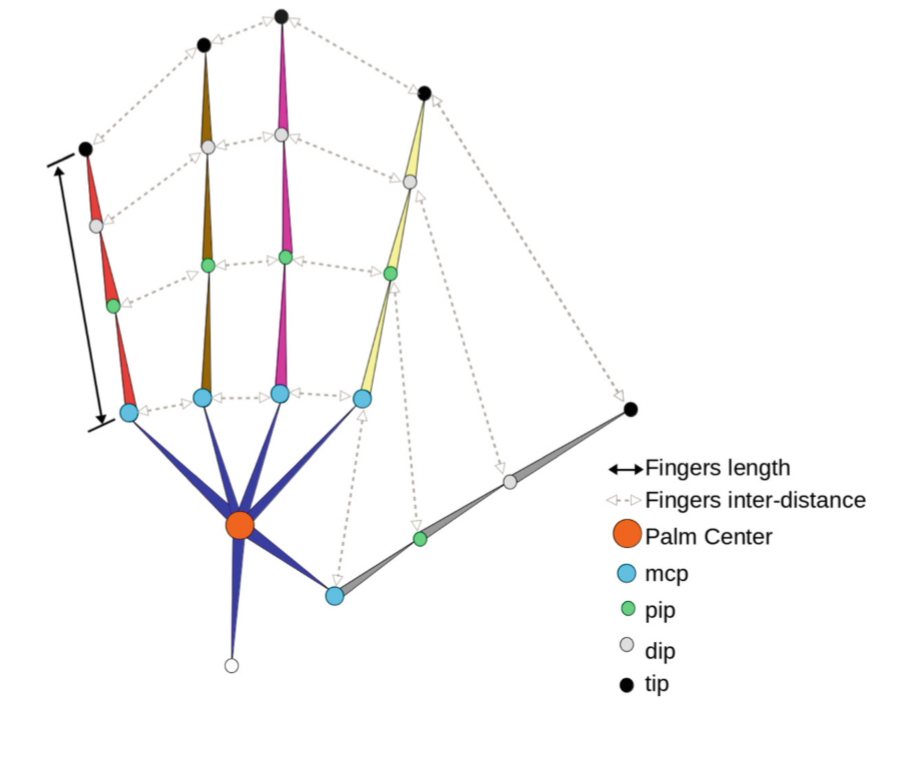
\includegraphics[width=0.7\linewidth]{Ressourcen/malik2018_hand_model}
		\caption[Handmodell nach \cite{Malik2018b}]{In \cite{Malik2018b} wird ein Modell ähnlich dem oben stehenden (Quelle: \cite{Malik2018b}) genutzt, in dem die vollständige Handpose durch 21, bzw. 22 (Gelenk-) Koordinaten bestimmt ist.}
		\label{fig:malik2018handmodel}
	\end{figure}
	
	
	\subsection{title}
	